\documentclass{standalone}%
\usepackage[T1]{fontenc}%
\usepackage[utf8]{inputenc}%
\usepackage{lmodern}%
\usepackage{textcomp}%
\usepackage{lastpage}%
\usepackage{tikz}%
%
%
%
\begin{document}%
\normalsize%
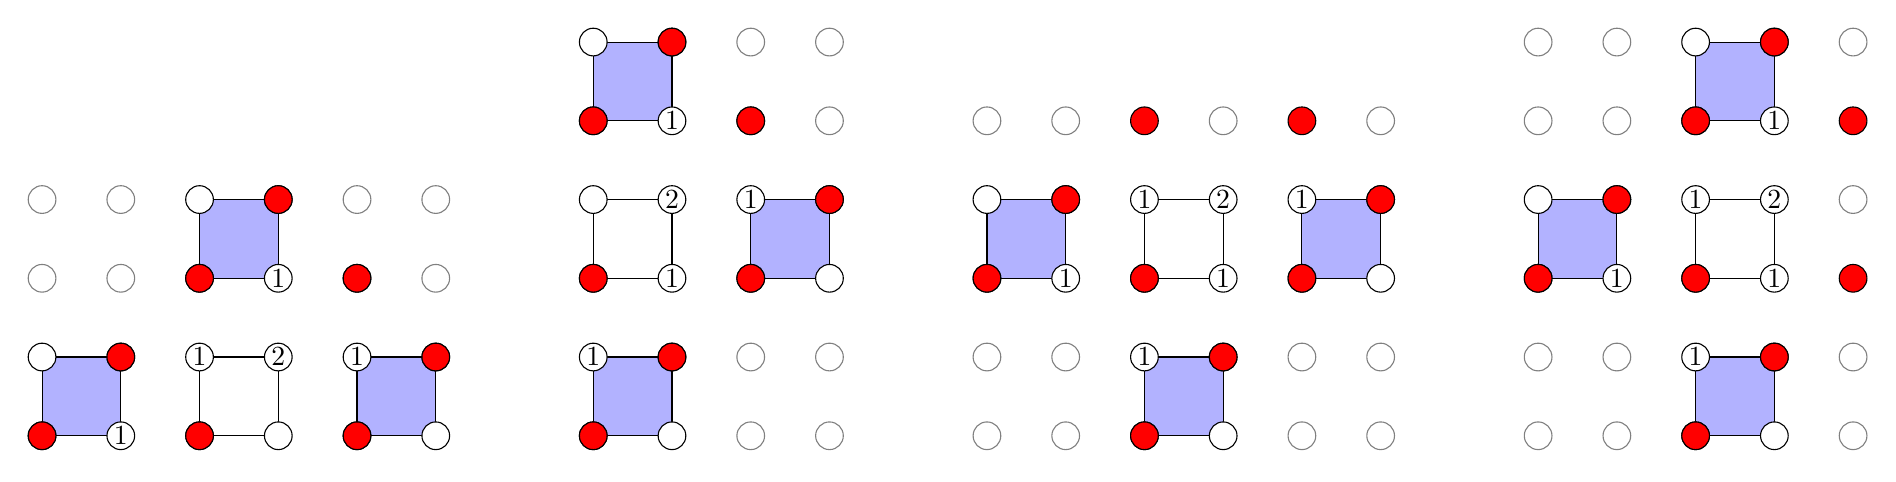
\begin{tikzpicture}[scale=1.0]%

\draw[fill=blue!30] (0,-5) rectangle (1,-4);
\draw[fill=blue!30] (2,-3) rectangle (3,-2);
\draw[fill=blue!30] (4,-5) rectangle (5,-4);
\draw[] (2,-5) rectangle (3,-4);

\draw[fill=blue!30] (7,-1) rectangle (8,0);
\draw[fill=blue!30] (9,-3) rectangle (10,-2);
\draw[fill=blue!30] (7,-5) rectangle (8,-4);
\draw[] (7,-3) rectangle (8,-2);

\draw[fill=blue!30] (12,-3) rectangle (13,-2);
\draw[fill=blue!30] (14,-5) rectangle (15,-4);
\draw[fill=blue!30] (16,-3) rectangle (17,-2);
\draw[] (14,-3) rectangle (15,-2);

\draw[fill=blue!30] (21,-1) rectangle (22,0);
\draw[fill=blue!30] (19,-3) rectangle (20,-2);
\draw[fill=blue!30] (21,-5) rectangle (22,-4);
\draw[] (21,-3) rectangle (22,-2);

\path[draw,radius=5pt, fill=white] (7.0,0.0) circle;%
\path[draw,radius=5pt, fill=white] (8.0,0.0) circle;%
\path[draw,radius=5pt, gray,fill=white] (9.0,0.0) circle;%
\path[draw,radius=5pt, gray,fill=white] (10.0,0.0) circle;%
\path[draw,radius=5pt, gray,fill=white] (19.0,0.0) circle;%
\path[draw,radius=5pt, gray,fill=white] (20.0,0.0) circle;%
\path[draw,radius=5pt, fill=white] (21.0,0.0) circle;%
\path[draw,radius=5pt, fill=white] (22.0,0.0) circle;%

\path[draw,radius=5pt, fill=white] (7.0,-1.0) circle;%
\path[draw,radius=5pt, fill=white] (8.0,-1.0) circle;%
\path[draw,radius=5pt, fill=white] (9.0,-1.0) circle;%
\path[draw,radius=5pt,gray, fill=white] (10.0,-1.0) circle;%
\path[draw,radius=5pt, gray,fill=white] (19.0,-1.0) circle;%
\path[draw,radius=5pt, gray,fill=white] (20.0,-1.0) circle;%
\path[draw,radius=5pt, fill=white] (21.0,-1.0) circle;%
\path[draw,radius=5pt, fill=white] (22.0,-1.0) circle;%

\path[draw,radius=5pt, gray,fill=white] (0.0,-2.0) circle;%
\path[draw,radius=5pt, gray,fill=white] (1.0,-2.0) circle;%
\path[draw,radius=5pt, fill=white] (2.0,-2.0) circle;%
\path[draw,radius=5pt, fill=white] (3.0,-2.0) circle;%
\path[draw,radius=5pt, gray,fill=white] (4.0,-2.0) circle;%
\path[draw,radius=5pt, gray,fill=white] (5.0,-2.0) circle;%
\path[draw,radius=5pt, fill=white] (7.0,-2.0) circle;%
\path[draw,radius=5pt, fill=white] (8.0,-2.0) circle;%
\path[draw,radius=5pt, fill=white] (9.0,-2.0) circle;%
\path[draw,radius=5pt, fill=white] (10.0,-2.0) circle;%
\path[draw,radius=5pt, fill=white] (12.0,-2.0) circle;%
\path[draw,radius=5pt, fill=white] (13.0,-2.0) circle;%
\path[draw,radius=5pt, fill=white] (14.0,-2.0) circle;%
\path[draw,radius=5pt, fill=white] (15.0,-2.0) circle;%
\path[draw,radius=5pt, fill=white] (16.0,-2.0) circle;%
\path[draw,radius=5pt, fill=white] (17.0,-2.0) circle;%
\path[draw,radius=5pt, fill=white] (19.0,-2.0) circle;%
\path[draw,radius=5pt, fill=white] (20.0,-2.0) circle;%
\path[draw,radius=5pt, fill=white] (21.0,-2.0) circle;%
\path[draw,radius=5pt, fill=white] (22.0,-2.0) circle;%

\path[draw,radius=5pt, gray,fill=white] (0.0,-3.0) circle;%
\path[draw,radius=5pt, gray,fill=white] (1.0,-3.0) circle;%
\path[draw,radius=5pt, fill=white] (2.0,-3.0) circle;%
\path[draw,radius=5pt, fill=white] (3.0,-3.0) circle;%
\path[draw,radius=5pt, fill=white] (4.0,-3.0) circle;%
\path[draw,radius=5pt, gray,fill=white] (5.0,-3.0) circle;%
\path[draw,radius=5pt, fill=white] (7.0,-3.0) circle;%
\path[draw,radius=5pt, fill=white] (8.0,-3.0) circle;%
\path[draw,radius=5pt, fill=white] (9.0,-3.0) circle;%
\path[draw,radius=5pt, fill=white] (10.0,-3.0) circle;%
\path[draw,radius=5pt, fill=white] (12.0,-3.0) circle;%
\path[draw,radius=5pt, fill=white] (13.0,-3.0) circle;%
\path[draw,radius=5pt, fill=white] (14.0,-3.0) circle;%
\path[draw,radius=5pt, fill=white] (15.0,-3.0) circle;%
\path[draw,radius=5pt, fill=white] (16.0,-3.0) circle;%
\path[draw,radius=5pt, fill=white] (17.0,-3.0) circle;%
\path[draw,radius=5pt, fill=white] (19.0,-3.0) circle;%
\path[draw,radius=5pt, fill=white] (20.0,-3.0) circle;%
\path[draw,radius=5pt, fill=white] (21.0,-3.0) circle;%
\path[draw,radius=5pt, fill=white] (22.0,-3.0) circle;%

\path[draw,radius=5pt, fill=white] (0.0,-4.0) circle;%
\path[draw,radius=5pt, fill=white] (1.0,-4.0) circle;%
\path[draw,radius=5pt, fill=white] (2.0,-4.0) circle;%
\path[draw,radius=5pt, fill=white] (3.0,-4.0) circle;%
\path[draw,radius=5pt, fill=white] (4.0,-4.0) circle;%
\path[draw,radius=5pt, fill=white] (5.0,-4.0) circle;%
\path[draw,radius=5pt, fill=white] (7.0,-4.0) circle;%
\path[draw,radius=5pt, fill=white] (8.0,-4.0) circle;%
\path[draw,radius=5pt, gray,fill=white] (9.0,-4.0) circle;%
\path[draw,radius=5pt, gray,fill=white] (10.0,-4.0) circle;%
\path[draw,radius=5pt, gray,fill=white] (12.0,-4.0) circle;%
\path[draw,radius=5pt, gray,fill=white] (13.0,-4.0) circle;%
\path[draw,radius=5pt, fill=white] (14.0,-4.0) circle;%
\path[draw,radius=5pt, fill=white] (15.0,-4.0) circle;%
\path[draw,radius=5pt, gray,fill=white] (16.0,-4.0) circle;%
\path[draw,radius=5pt, gray,fill=white] (17.0,-4.0) circle;%
\path[draw,radius=5pt, gray,fill=white] (19.0,-4.0) circle;%
\path[draw,radius=5pt, gray,fill=white] (20.0,-4.0) circle;%
\path[draw,radius=5pt, fill=white] (21.0,-4.0) circle;%
\path[draw,radius=5pt, fill=white] (22.0,-4.0) circle;%

\path[draw,radius=5pt, fill=white] (0.0,-5.0) circle;%
\path[draw,radius=5pt, fill=white] (1.0,-5.0) circle;%
\path[draw,radius=5pt, fill=white] (2.0,-5.0) circle;%
\path[draw,radius=5pt, fill=white] (3.0,-5.0) circle;%
\path[draw,radius=5pt, fill=white] (4.0,-5.0) circle;%
\path[draw,radius=5pt, fill=white] (5.0,-5.0) circle;%
\path[draw,radius=5pt, fill=white] (7.0,-5.0) circle;%
\path[draw,radius=5pt, fill=white] (8.0,-5.0) circle;%
\path[draw,radius=5pt, gray,fill=white] (9.0,-5.0) circle;%
\path[draw,radius=5pt, gray,fill=white] (10.0,-5.0) circle;%
\path[draw,radius=5pt, gray,fill=white] (12.0,-5.0) circle;%
\path[draw,radius=5pt, gray,fill=white] (13.0,-5.0) circle;%
\path[draw,radius=5pt, fill=white] (14.0,-5.0) circle;%
\path[draw,radius=5pt, fill=white] (15.0,-5.0) circle;%
\path[draw,radius=5pt, gray,fill=white] (16.0,-5.0) circle;%
\path[draw,radius=5pt, gray,fill=white] (17.0,-5.0) circle;%
\path[draw,radius=5pt, gray,fill=white] (19.0,-5.0) circle;%
\path[draw,radius=5pt, gray,fill=white] (20.0,-5.0) circle;%
\path[draw,radius=5pt, fill=white] (21.0,-5.0) circle;%
\path[draw,radius=5pt, fill=white] (22.0,-5.0) circle;%
\path[draw,radius=5pt,fill=red] (8.0,0.0) circle;%
\path[draw,radius=5pt,fill=red] (22.0,0.0) circle;%
\path[draw,radius=5pt,fill=red] (7.0,-1.0) circle;%
\path[draw,radius=5pt,fill=red] (21.0,-1.0) circle;%
\path[draw,radius=5pt,fill=red] (3.0,-2.0) circle;%
\path[draw,radius=5pt,fill=red] (10.0,-2.0) circle;%
\path[draw,radius=5pt,fill=red] (13.0,-2.0) circle;%
\path[draw,radius=5pt,fill=red] (17.0,-2.0) circle;%
\path[draw,radius=5pt,fill=red] (20.0,-2.0) circle;%
\path[draw,radius=5pt,fill=red] (2.0,-3.0) circle;%
\path[draw,radius=5pt,fill=red] (4.0,-3.0) circle;%
\path[draw,radius=5pt,fill=red] (7.0,-3.0) circle;%
\path[draw,radius=5pt,fill=red] (9.0,-3.0) circle;%
\path[draw,radius=5pt,fill=red] (12.0,-3.0) circle;%
\path[draw,radius=5pt,fill=red] (14.0,-3.0) circle;%
\path[draw,radius=5pt,fill=red] (16.0,-3.0) circle;%
\path[draw,radius=5pt,fill=red] (19.0,-3.0) circle;%
\path[draw,radius=5pt,fill=red] (21.0,-3.0) circle;%
\path[draw,radius=5pt,fill=red] (1.0,-4.0) circle;%
\path[draw,radius=5pt,fill=red] (5.0,-4.0) circle;%
\path[draw,radius=5pt,fill=red] (8.0,-4.0) circle;%
\path[draw,radius=5pt,fill=red] (15.0,-4.0) circle;%
\path[draw,radius=5pt,fill=red] (22.0,-4.0) circle;%
\path[draw,radius=5pt,fill=red] (0.0,-5.0) circle;%
\path[draw,radius=5pt,fill=red] (2.0,-5.0) circle;%
\path[draw,radius=5pt,fill=red] (4.0,-5.0) circle;%
\path[draw,radius=5pt,fill=red] (7.0,-5.0) circle;%
\path[draw,radius=5pt,fill=red] (14.0,-5.0) circle;%
\path[draw,radius=5pt,fill=red] (21.0,-5.0) circle;%
\path[draw,radius=5pt,fill=red] (9,-1.0) circle;%

\path[draw,radius=5pt,fill=red] (14,-1.0) circle;%
\path[draw,radius=5pt,fill=red] (16,-1.0) circle;%
\path[draw,radius=5pt,fill=red] (23,-3.0) circle;%
\path[draw,radius=5pt,fill=red] (23,-1.0) circle;%

\path[draw,radius=5pt,gray] (12,-1.0) circle;%
\path[draw,radius=5pt,gray] (13,-1.0) circle;%
\path[draw,radius=5pt,gray] (15,-1.0) circle;%
\path[draw,radius=5pt,gray] (17,-1.0) circle;%

\path[draw,radius=5pt,gray] (23,0) circle;%
\path[draw,radius=5pt,gray] (23,-2) circle;%
\path[draw,radius=5pt,gray] (23,-4) circle;%
\path[draw,radius=5pt,gray] (23,-5) circle;%

\node at (1,-5) {$1$};
\node at (2,-4) {$1$};
\node at (3,-3) {$1$};
\node at (4,-4) {$1$};
\node at (3,-4) {$2$};

\node at (7,-4) {$1$};
\node at (8,-3) {$1$};
\node at (9,-2) {$1$};
\node at (8,-1) {$1$};
\node at (8,-2) {$2$};

\node at (13,-3) {$1$};
\node at (14,-4) {$1$};
\node at (15,-3) {$1$};
\node at (14,-2) {$1$};
\node at (16,-2) {$1$};
\node at (15,-2) {$2$};

\node at (20,-3) {$1$};
\node at (21,-4) {$1$};
\node at (22,-3) {$1$};
\node at (21,-2) {$1$};
\node at (22,-1) {$1$};
\node at (22,-2) {$2$};

\end{tikzpicture}%
\end{document}